\documentclass[11pt]{article} 
\usepackage[english]{babel}
\usepackage[utf8]{inputenc}
\usepackage[margin=0.5in]{geometry}
\usepackage{amsmath}
\usepackage{amsthm}
\usepackage{amsfonts}
\usepackage{amssymb}
\usepackage[usenames,dvipsnames]{xcolor}
\usepackage{graphicx}
\usepackage[siunitx]{circuitikz}
\usepackage{tikz}
\usepackage{tkz-berge}
\usetikzlibrary{positioning, automata, backgrounds}
\usepackage[colorinlistoftodos, color=orange!50]{todonotes}
\usepackage{hyperref}
\usepackage[numbers, square]{natbib}
\usepackage{fancybox}
\usepackage{epsfig}
\usepackage{soul}
\usepackage[framemethod=tikz]{mdframed}
\usepackage[shortlabels]{enumitem}
\usepackage[version=4]{mhchem}
\usepackage{multicol}
\usepackage{forest}
\usepackage{mathtools}
\usepackage{comment}
\usepackage{enumitem}
\usepackage[utf8]{inputenc}
\usepackage{listings}
\usepackage{color}
\usepackage[numbers]{natbib}
\usepackage{subfiles}
\usepackage{tkz-berge}
\usepackage{algorithm}
\usepackage[noend]{algpseudocode}


\newtheorem{prop}{Proposition}[section]
\newtheorem{thm}{Theorem}[section]
\newtheorem{lemma}{Lemma}[section]
\newtheorem{cor}{Corollary}[prop]

\theoremstyle{definition}
\newtheorem{definition}{Definition}

\theoremstyle{definition}
\newtheorem{required}{Problem}

\theoremstyle{definition}
\newtheorem{ex}{Example}

\newcommand{\interval}[4]{\draw (#2, #1) -- (#3, #1); % Usage: \interval{height}{start}{end}{label}
\draw (#2, #1-0.11) -- (#2, #1+0.11); % draw left whisker
\draw (#3, #1-0.11) -- (#3, #1+0.11); % draw right whisker
\node[] at (#2-0.25, #1) {#4};
}


\setlength{\marginparwidth}{3.4cm}
%#########################################################

%To use symbols for footnotes
\renewcommand*{\thefootnote}{\fnsymbol{footnote}}
%To change footnotes back to numbers uncomment the following line
%\renewcommand*{\thefootnote}{\arabic{footnote}}

% Enable this command to adjust line spacing for inline math equations.
% \everymath{\displaystyle}

% _______ _____ _______ _      ______ 
%|__   __|_   _|__   __| |    |  ____|
%   | |    | |    | |  | |    | |__   
%   | |    | |    | |  | |    |  __|  
%   | |   _| |_   | |  | |____| |____ 
%   |_|  |_____|  |_|  |______|______|
%%%%%%%%%%%%%%%%%%%%%%%%%%%%%%%%%%%%%%%

\title{
\normalfont \normalsize 
\textsc{CSCI 3104 Fall 2021 \\ 
Instructors: Profs. Grochow and Waggoner} \\
[10pt] 
\rule{\linewidth}{0.5pt} \\[6pt] 
\huge Problem Set 8\\
\rule{\linewidth}{2pt}  \\[10pt]
}
%\author{Your Name}
\date{}

\begin{document}
\definecolor {processblue}{cmyk}{0.96,0,0,0}
\maketitle


%%%%%%%%%%%%%%%%%%%%%%%%%
%%%%%%%%%%%%%%%%%%%%%%%%%%
%%%%%%%%%%FILL IN YOUR NAME%%%%%%%
%%%%%%%%%%AND STUDENT ID%%%%%%%%
%%%%%%%%%%%%%%%%%%%%%%%%%%
\noindent
Due Date \dotfill TODO \\
Name \dotfill \textbf{Didi Trifonova} \\
Student ID \dotfill \textbf{109388776} \\
Collaborators \dotfill \textbf{Maria Garcia}

\tableofcontents

\section{Instructions}
 \begin{itemize}
	\item The solutions \textbf{must be typed}, using proper mathematical notation. We cannot accept hand-written solutions. \href{http://ece.uprm.edu/~caceros/latex/introduction.pdf}{Here's a short intro to \LaTeX.}
	\item You should submit your work through the \textbf{class Canvas page} only. Please submit one PDF file, compiled using this \LaTeX \ template.
	\item You may not need a full page for your solutions; pagebreaks are there to help Gradescope automatically find where each problem is. Even if you do not attempt every problem, please submit this document with no fewer pages than the blank template (or Gradescope has issues with it).

	\item You are welcome and encouraged to collaborate with your classmates, as well as consult outside resources. You must \textbf{cite your sources in this document.} \textbf{Copying from any source is an Honor Code violation. Furthermore, all submissions must be in your own words and reflect your understanding of the material.} If there is any confusion about this policy, it is your responsibility to clarify before the due date. 

	\item Posting to \textbf{any} service including, but not limited to Chegg, Reddit, StackExchange, etc., for help on an assignment is a violation of the Honor Code.

	\item You \textbf{must} virtually sign the Honor Code (see Section \ref{HonorCode}). Failure to do so will result in your assignment not being graded.
\end{itemize}


\section{Honor Code (Make Sure to Virtually Sign)} \label{HonorCode}

\begin{required}
\begin{itemize}
\item My submission is in my own words and reflects my understanding of the material.
\item Any collaborations and external sources have been clearly cited in this document.
\item I have not posted to external services including, but not limited to Chegg, Reddit, StackExchange, etc.
\item I have neither copied nor provided others solutions they can copy.
\end{itemize}

%\noindent In the specified region below, clearly indicate that you have upheld the Honor Code. Then type your name. 
\end{required}

\begin{proof}[Agreed (Didi Trifonova).]
%% Typing "I agree to the above," followed by your name is sufficient.
\end{proof}


\newpage
\section{Standard 21- Dynamic Programming: Identify the Precise Subproblems}

\noindent The goal of this standard is to practice identifying the recursive structure. To be clear, you are \textbf{not} being asked for a precise mathematical recurrence. Rather, you are being asked to clearly and precisely identify the cases to consider. Identifying the cases can sometimes provide enough information to design a dynamic programming solution.

\subsection{Problem \ref{DP1}}
\begin{required} \label{DP1}
Consider the \textsf{Stair Climbing} problem, defined as follows.
\begin{itemize}
\item \textsf{Instance:} Suppose we have $n$ stairs, labeled $s_{1}, \ldots, s_{n}$. Each stair $s_{k}$ has a number $a_{k} \geq 1$ associated to it. At stair $s_{k}$, we may jump forward $i$ stairs, where $i \in \{ 1, 2, \ldots, a_{k}\}$. You start on $s_{1}$.

\item \textsf{Solution:} The number of ways to to reach $s_{n}$ from $s_{1}$.
\end{itemize}

\noindent \\ \textbf{Your job} is to clearly identify the recursive structure. That is, suppose we are solving the subproblem at stair $s_{k}$. What precise sub-problems do we need to consider?
\end{required}

\begin{proof}[Answer] $ $\\
\textbf{Subproblem} - Stairs you can reach with one jump when starting at $s_k$, beginning with $k=1$ to $k=n$. \\ The base case for this problem is $s_1$ because that is the stair that you start on. An example of this subproblem is if we are on $s_2$ and $a_2$ has a value of 2. That means that from stair $s_2$ we can jump to either $s_3$ or $s_4$. 
\end{proof}



\newpage
\subsection{Problem \ref{DP2}}
\begin{required} \label{DP2}
Fix $n \in \mathbb{N}$. The \textit{Trust Game} on $n$ rounds is a two-player dynamic game. Here, Player I starts with \$100. The game proceeds as follows.
\begin{itemize}
\item \textbf{Round 1:} Player I takes a fraction of the \$100 (which could be nothing) to give to Player II. The money Player I gives to Player II is multiplied by 1.5 before Player II receives it. Player I keeps the remainder. (So for example, if Player I gives \$20 to Player II, then Player II receives \$30 and Player I is left with \$80).

\item \textbf{Round 2:} Player II can choose a fraction of the money they received to offer to Player I. The money offered to Player I increases by a multiple of $1.5$  before Player I receives it. Player II keeps the remainder.
\end{itemize}

\noindent \\ More generally, at round $i$, the Player at the current round (Player I if $i$ is odd, and Player II if $i$ is even) takes a fraction of the money in the current pile to send to the other Player and keeps the rest. That money increases by a factor of $1.5$ before the other player receives it. The game terminates if the current player does not send any money to the other player, or if round $n$ is reached. At round $n$, the money in the pile is split evenly between the two players. \\

\noindent Each individual player wishes to maximize the total amount of money they receive. \\

\noindent \textbf{Your job} is to clearly identify the recursive structure. That is, at round $i$, what precise sub-problems does the current player need to consider? [\textbf{Hint:} Do we have a smaller instance of the Trust Game after each round?]
\end{required}

\begin{proof}[Answer]
At round i, the current player needs to consider how much money is left in the pile after the i-1 round. They also need to consider how much money they've accumulated after the i-2 round. Finally they need to consider how much money will be in the pile at the end of the i round if they take m amount of money. They would also need to add m amount of money to their total from i-2 round. 
\end{proof}




\newpage
\section{Standard 22- Dynamic Programming: Write Down Recurrences}

\subsection{Problem \ref{DP3}}

\begin{required} \label{DP3}
Suppose we have an $m$-letter alphabet $\Sigma = \{0, 1, \ldots, m-1\}$. Let $W_{n}$ be the set of strings $\omega \in \Sigma^{n}$ such that $\omega$ does not have $00$ as a substring. Let $f_{n} := |W_{n}|$. Write down an explicit recurrence for $f_{n}$, including the base cases. Clearly justify each recursive term.
\end{required}

\begin{proof}[Answer]
\begin{equation}
  f(n)=\begin{cases}
    1 & n=0\\
    m & n=1 \\
    f_{n-1}(m-1) + f_{n-2}(m-1) & n\geq 2
  \end{cases}
\end{equation} \\
This recurrence relation comes from the fact that there are two disjoint cases to consider. \\ \\
\textbf{Case 1: }This case is when the string does not end with a zero. With a string of length n, there are $(m-1)$ possibilities for the last entry because it can be anything but zero. To find all the possibilities for this case, it can be multiplied by the number of possibilities of length $n-1$, which is simply $f_{n-1}(m-1)$ \\ \\
\textbf{Case 2: }This case is when the string ends with a zero. This means the last entry has 1 possibility, zero. The n-1 entry, however, will have $(m-1)$ possibilities because it cannot be 0. Then this can be multiplied by the number of possibilities for a string of n-2 length. The number of possibilities for this case is $f_{n-2}(m-1)\cdot 1$. These cases are disjoint, therefore we can add them together to get our recurrence relation. \\ \\
\textbf{Base cases: }When the length is 0, there is one possibility for $W_n$ which is the empty set. When the length is 1, the entry can be any of m letters, therefore having m possibilites. 
\end{proof}

%You may find the following commented code helpful in rendering a recurrence
\begin{comment}
\begin{align*}
f_{n} &= \begin{cases} \text{Case1} & : \text{Condition1}, \\ 
\text{Case2} & : \text{Condition2}. 
\end{cases}
\end{align*}
\end{comment}




\newpage
\subsection{Problem \ref{DP4}}

\begin{required} \label{DP4}
Suppose we have the alphabet $\Sigma = \{x, y\}$. For $n \geq 0$, let $W_{n}$ be the set of strings $\omega \in \{x, y\}^{n}$ where $\omega$ contains $yyy$ as a substring. Let $f_{n} := |W_{n}|$. Write down an explicit recurrence for $f_{n}$, including the base cases. Clearly justify each recursive term.
\end{required}

\begin{proof}[Answer]
\begin{equation}
  f(n)=\begin{cases}
    0 & n < 3\\
    1 & n=3 \\
    f_{n-1} + f_{n-2} + f_{n-3} + 2^{n-3} & n > 3
  \end{cases}
\end{equation} \\
\textbf{Base cases: }If $n<3$ then it is not possible to create the string yyy. If $n=3$ then there is only one possibility, yyy.  \\ \\
\textbf{Case 1: }The first case is when the string ends in an x. Here we simply look to $f_{n-1}$ for the number of possibilities. \\ \\
\textbf{Case 2:} The string ends in a $y$. If this is the case we check the $n-1$ position and if it is an $x$ then we look at $f_{n-2}$ for our answer. If it is another $y$ then we must check the $n-2$ position. If there is an $x$ then look at $f_{n-3}$ for the answer. If there is a y then that means there are 3 consecutive y values and the other $n-3$ values can be any combination, which gives us $2^{n-3}$ possibilites. 
\end{proof}




\newpage
\section{Standard 23- Dynamic Programming: Using Recurrences to Solve}

\subsection{Problem \ref{Recurrence1}}
\begin{required} \label{Recurrence1}
Given the following directed acyclic graph. Use dynamic programming to fill in a \textbf{one-dimensional} lookup table that counts number of paths from each node $j$ to 14, for $j \geq 1$. Note that a single vertex is considered a path of length $0$. \textbf{Fill in the lookup table for all vertices 1-14; and in addition, clearly show work for vertices 9-14}.

        % ----- FIGURE -----
        \begin{figure}[h!]
        \begin{center}
        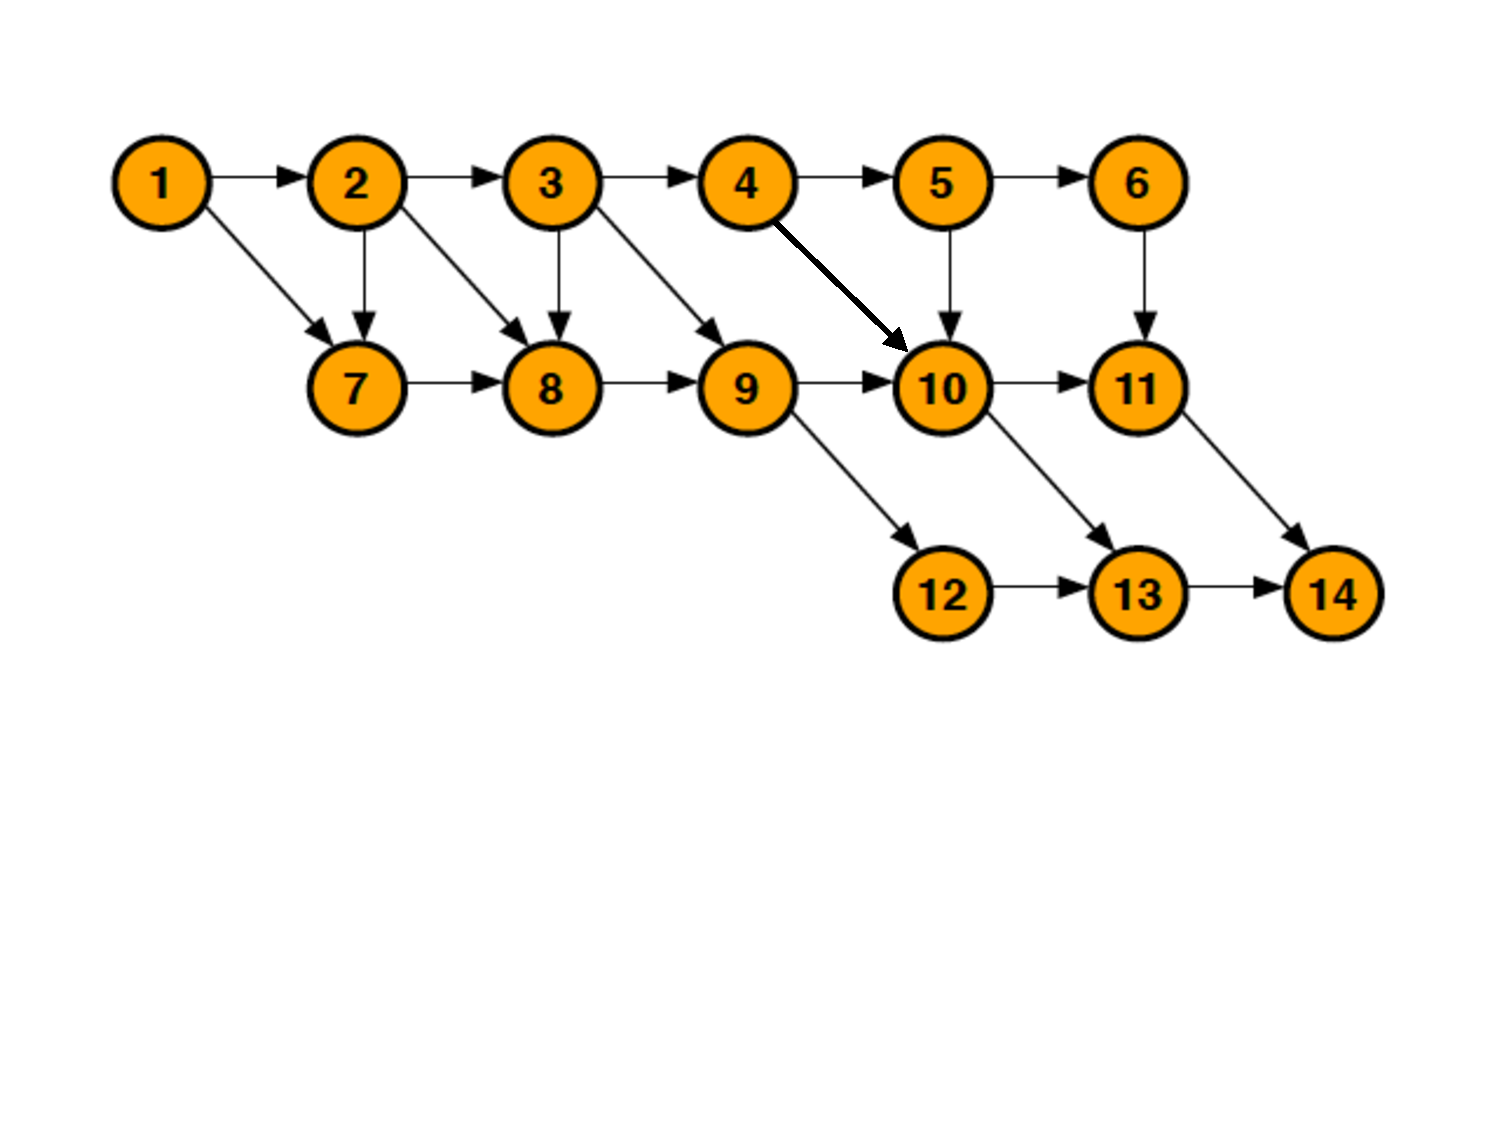
\includegraphics[scale=0.45]{dag_ps10.pdf} 
        \end{center}
        \end{figure}
        % ----------

\end{required}


\begin{proof}[Answer]
Topological sort: 1,2,3,4,5,6,7,8,9,10,11,12,13,14  \\
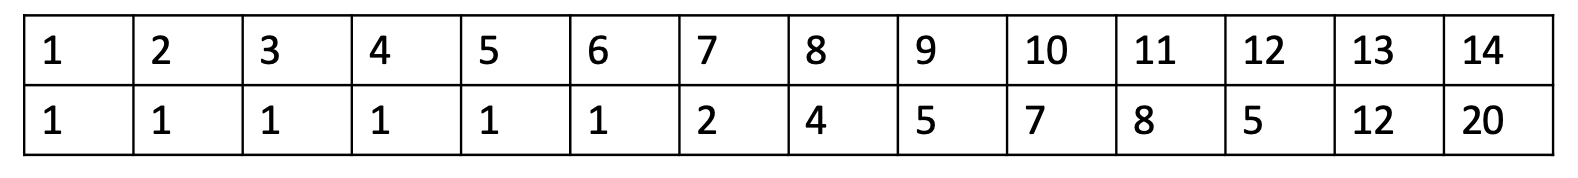
\includegraphics[width = 170mm]{lookup.png} \\
\begin{itemize}
    \item Vertex 9:  Predecessors are 3 and 8. A[3] + A[8] = (1 + 4) = 5 =  A[9]
    \item Vertex 10: Predecessors are 4, 5, and 9. A[4] + A[5] + A[9] = (1+1+5) = 7 = A[10]
    \item Vertex 11: Predecessors are 6 and 10. A[6] + A[10] = (1+7) = 8 = A[11]
    \item Vertex 12: Predecessor is 9. A[9] = 5 = A[12]
    \item Vertex 13: Predecessors are 10 and 12. A[10] + A[12]  = (7+5) = 12 = A[13]
    \item Vertex 14: Predecessors are 11 and 13. A[11] + A[13] = (8+12) = 20 = A[14]
    
\end{itemize}
\end{proof}




\newpage
\subsection{Problem \ref{Recurrence2}}
\begin{required} \label{Recurrence2}
Suppose we wish to multiply an $n \times m$ and $m \times k$ matrix. This operation takes $nmk$ multiplications. Consider the \textsf{Matrix Product} problem, which defined as follows.
\begin{itemize}
\item \textsf{Instance:} Matrices $A_{1}, \ldots, A_{n}$ with integer entries, where $A_{i}$ has dimensions $n_{i} \times m_{i}$. Note that for $1 \leq i < n$, we necessarily have that $m_{i} = n_{i+1}$.

\item \textsf{Solution:} Compute $A_{1}A_{2} \cdots A_{n}$, using the minimum number of integer multiplications.
\end{itemize}


\noindent \\ We note that matrix multiplication is associative; that is, $A(BC) = (AB)C$. So we may parenthesize $A_{1}A_{2} \cdots A_{n}$ however we wish, without changing the expression. Certain parenthesizations require fewer multiplications than others. For instance, suppose $A$ is a $10 \times 30$ matrix, $B$ is a $30 \times 5$ matrix, and $C$ is a $5 \times 60$ matrix. Observe that $A(BC)$ requires $(10 \cdot 30 \cdot 60) + (30 \cdot 60 \cdot 5) = 27000$ multiplications, while $(AB)C$ requires $(30 \cdot 5 \cdot 10) + (10 \cdot 5 \cdot 60) = 4500$ multiplications. \\

\noindent For $1 \leq i \leq j \leq n$, denote $m[i, j]$ as the minimum number of multiplications required to evaluate $A_{i} \cdots A_{j}$. Note that $m[i, j]$ is given by the following recurrence:
\[
m[i, j] = \begin{cases} 
0 & : i = j, \\
\displaystyle \min_{i \leq k < j} (m[i, k] + m[k+1, j] + n_{i}m_{k}m_{j}) & : i < j.
\end{cases}
\]

\noindent Here, we have that:
\begin{itemize}
\item $m[i, k]$ is the minimum number of multiplications to compute $M_{1} := A_{i} \cdots A_{k}$. Note that $M_{1}$ is an $n_{i} \times m_{k}$ matrix.

\item $m[k+1, j]$ is the minimum number of multiplications to compute $M_{2} := A_{k+1} \cdots A_{j}$. Note that $M_{2}$ is an $m_{k} \times m_{j}$ matrix (here, $m_{k} = n_{k+1}$).

\item $n_{i}m_{k}m_{j}$ is the number of multiplications required to compute $M_{1} \cdot M_{2}$. 
\end{itemize}


\noindent \\ \textbf{Your job} is as follows. Suppose we are given matrices of the following dimension:
\begin{itemize}
\item $A_{1}$: $2 \times 8$.
\item $A_{2}$: $8 \times 9$.
\item $A_{3}$: $9 \times 10$.
\item $A_{4}$: $10 \times 20$.
\item $A_{5}$: $20 \times 6$.
\end{itemize}

\noindent \\ Design and fill in a 2D lookup table to compute the minimum number of integer multiplications required to compute $A_{1} \cdots A_{5}$. Include the optimal back pointers. [\textbf{Note:} You may hand-draw and embed your lookup table, provided it is legible and we do not have to rotate our screens to read it. All other accompanying work \textbf{must} be typed.]
\end{required}

\begin{proof}[Answer] 
\begin{align*}
    m[1,2] &= min( m[1,1] + m[2,2] + (2\cdot8\cdot9)) = 144 \\
    m[2,3] &= min( m[2,2] + m[3,3] + (8\cdot9\cdot10)) = 720 \\
    m[3,4] &= min( m[3,3] + m[4,4] + (9\cdot10\cdot20)) = 1800 \\
    m[4,5] &= min( m[4,4] + m[5,5] + (6\cdot10\cdot20)) = 1200 \\
    m[1,3] &= min((m[1,1] + m[2,3] + 2\cdot8\cdot10), (m[1,2] + m[3,3] + 2\cdot9\cdot10))\\ &= min((0+720+160), (144+0+180)) =  min((880, 324) = 324 \\
    m[2,4] &= min((m[2,2]+m[3,4] +8\cdot9\cdot20 ),(m[2,3] + m[4,4] + 8\cdot10\cdot20)) \\
    &= min((0+1800+1440),(720+0+1600)) = min(3240, 2320) = 2320 \\
    m[3,5] &= min((m[3,3] + m[4,5] + 9\cdot10\cdot6),(m[3,4] + [5,5] + 9\cdot20\cdot6)) \\
    &= min((0+1200+540),(1800+0+1080)) = min(1740, 2880) = 1740 \\
    m[1,4] &= min((m[1,1]+m[2,4]+2\cdot8\cdot20),(m[1,2]+m[3,4]+2\cdot9\cdot20),(m[1,3]+m[4,4]+2\cdot10\cdot20))    \\
    &= min((0+2320+320),(144+1800+360),(324+0+400)) = min(2640,2304,724) = 724 \\
    m[2,5] &= min((m[2,2]+m[3,5]+8\cdot9\cdot6),(m[2,3]+m[4,5]+8\cdot10\cdot6),(m[2,4]+m[5,5]+8\cdot20\cdot6)) \\
    &= min((0+1740+432),(720+1200+480),(2320+0+960)) = min(2172,2400,3280) = 2172 \\
    m[1,5] &= min((m[1,1]+m[2,5]+96),(m[1,2]+[3,5]+108),(m[1,3]+m[4,5]+120),(m[1,4]+m[5,5]+240)) \\
    &= min((0+2172+96),(144+1740+108),(324+1200+120),(724+0+240))\\ &= (2268,1992,1644,964) =964
\end{align*}
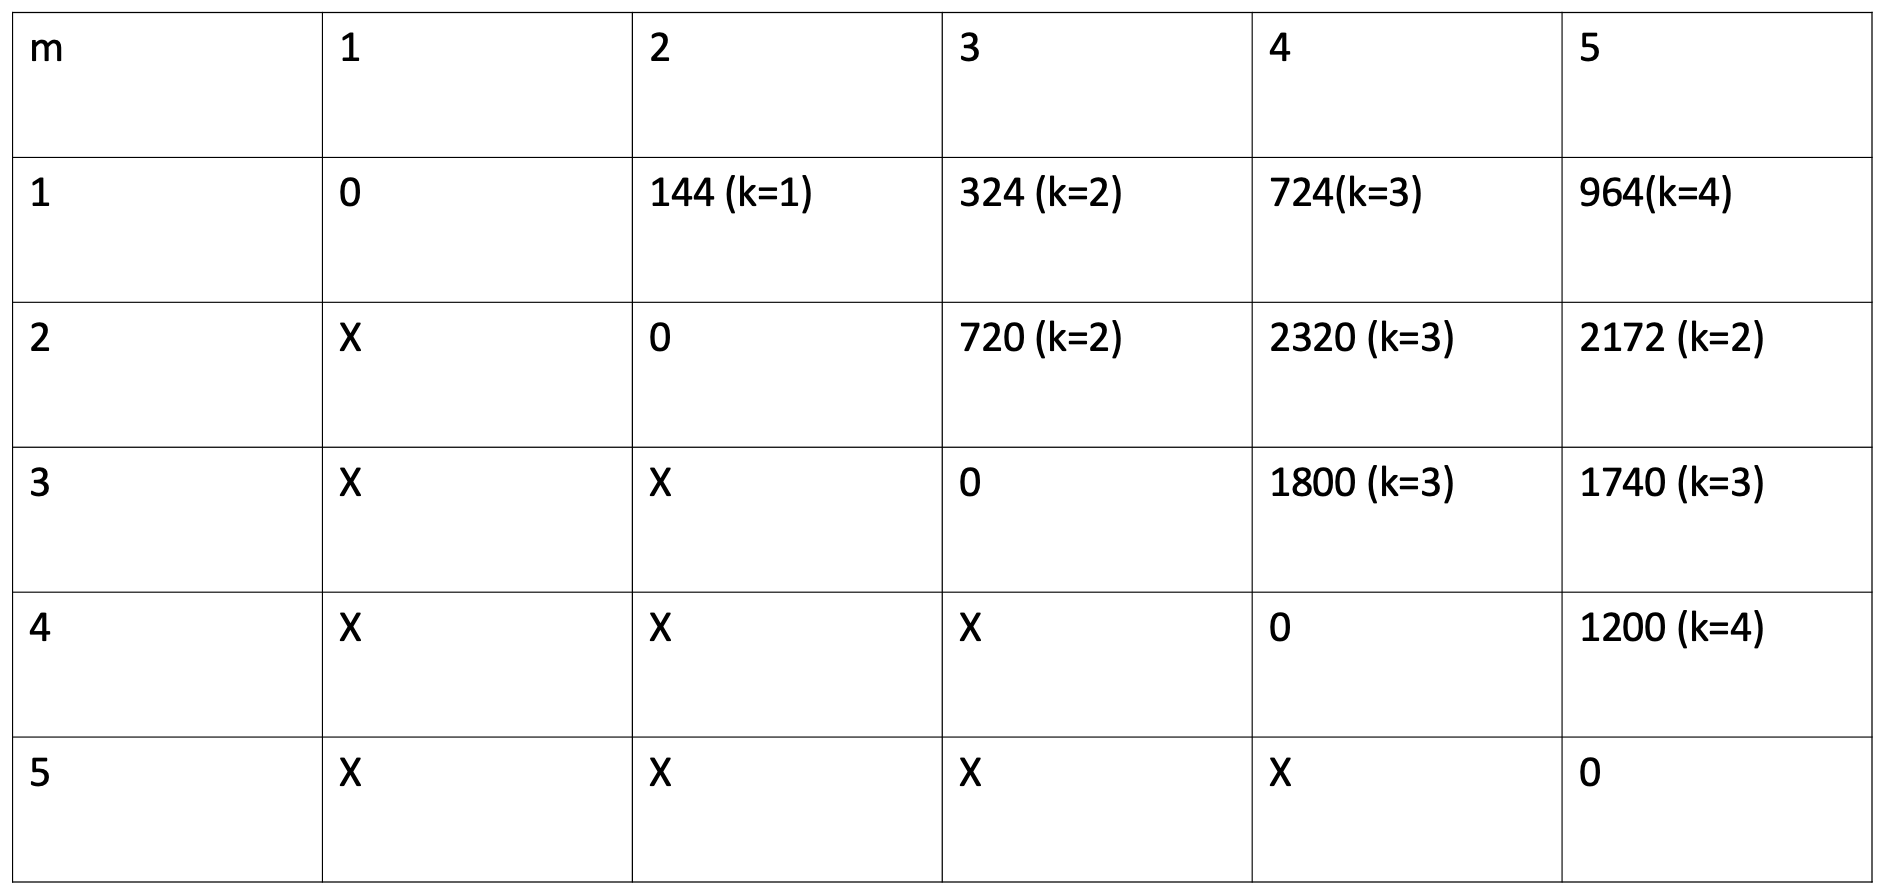
\includegraphics[width = 190mm]{2d.png}
\end{proof}

\end{document} % NOTHING AFTER THIS LINE IS PART OF THE DOCUMENT



